% vim: set spell spelllang=es syntax=tex :

\documentclass[11pt,a4paper,spanish]{beamer}

\usepackage[spanish]{babel}

\usepackage[utf8]{inputenc}

\usepackage{graphicx}

\usepackage{subcaption} %Para Subfigure

\usepackage{caption} %Para captions en las figuras sin prefijo

\usepackage{ccicons}

\usepackage{url}

\usepackage{babelbib}

\usepackage{textcomp}

\usepackage{tabularx}

\usepackage{styles/egyptian}

\newcommand{\aprox}{\raisebox{0.5ex}{\texttildelow}}
\newcommand{\bit}{\textbf{b}}
\newcommand{\Byte}{\textbf{B}}

\newcommand{\multiline}[2][c]{
      \begin{tabular}[#1]{@{}c@{}}#2\end{tabular}
      }


\usefonttheme{serif}

\setlength{\parskip}{1.5mm}

\usetheme{Rochester}
\usecolortheme{whale}

%\usetheme{Warsaw}

\beamertemplatenavigationsymbolsempty

\setbeamertemplate{background canvas}{
    \raisebox{-0.99\paperheight}[0pt][0pt]{
        \makebox[\paperwidth]{
            \null
            \hspace{-1em}
            \includegraphics[width=0.09\paperwidth]{logos/fai.pdf}
            \hspace{0.8\paperwidth}
            \hspace{-0.5em}
            \includegraphics[width=0.09\paperwidth]{logos/uncoma.pdf}
            }
    }
}

\defbeamertemplate{footline}{centered page number}
{
    \hspace*{\fill}
    \usebeamercolor[fg]{blue}
    \usebeamerfont{page number in head/foot}
    \insertpagenumber\,/\,\insertpresentationendpage
    \hspace*{\fill}\vskip2pt
}
\setbeamertemplate{footline}[centered page number]

\title{Seguridad de nivel de Infraestructura en Sistemas Computacionales}
\author{}
\date{}

\begin{document}

\begin{frame}[noframenumbering]


    \maketitle
    \centering
    %\vspace{-8em}~
    %\begin{figure}
    %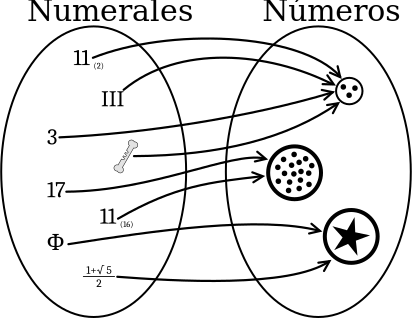
\includegraphics[height=0.65\textheight]{img/numerales.pdf}
        %\captionsetup{textfont=tiny,labelformat=empty,justification=centering}
        %\caption{}
    %\end{figure}

\end{frame}

\begin{frame}

    \frametitle{Temario}

\begin{itemize}

    \item ¿Qué es seguridad a nivel de infraestructura?
    \item Seguridad física: 
    \begin{itemize}
        \item Desastres naturales.
        \item Control de acceso.
    \end{itemize}
    \item Seguridad lógica:
    \begin{itemize}
        \item Seguridad de red.
        \item Protección de datos.
    \end{itemize}
    \item Vigilancia.

\end{itemize}
\end{frame}

\begin{frame}
    \frametitle{¿Qué es seguridad a nivel de infraestructura?}

    La seguridad a nivel de infraestructura es aquella que tiene como objetivo
    proteger a los componentes físicos y lógicos de los sistemas de
    computo.

    \begin{itemize}
        \item Seguridad física: mantener la integridad de los dispositivos de
            hardware.
        \item Seguridad lógica: protección de los datos almacenados y en
            transito.
    \end{itemize}
\end{frame}

\begin{frame}
    \frametitle{Seguridad física}
    \framesubtitle{Desastres naturales}
    
    \begin{itemize}
        \item Fuego y humo.
        \item Temperatura y humedad.
        \item Agua.
        \item Terremotos y
            vibración\footnote{\url{https://devblogs.microsoft.com/oldnewthing/20220816-00/?p=106994}}.
        \item Electricidad.
    \end{itemize}
\end{frame}

\begin{frame}
    \frametitle{Seguridad física}
    \framesubtitle{Control de acceso}

    ``La primer linea de defensa contra los intrusos es que no puedan entrar a
    tu edificio ni sala de computadoras'' ---\emph{Computer Security Basics,
    O'Reilly \& Associates, Inc.}
    
    Las cerraduras solo deberían dejar pasar a alguien pase un test de
    \emph{autentificación}. Los tres métodos para autentificarse son:
    \begin{itemize}
        \item Por algo que conoces \emph(ej. una contraseña).
        \item Por algo que tiene \emph(ej. una llave, un generador de tokens).
        \item Por algo que eres \emph(ej. escaneo de retina).
    \end{itemize}
\end{frame}

\begin{frame}
    \frametitle{Seguridad lógica}
    \framesubtitle{Seguridad de red}
    
    \begin{itemize}
        \item Mantener la integridad y privacidad de los datos en transito.
        \item Asegurar que se mantenga el servicio de red.
        \item Separar redes seguras de aquellas de las publicas.
        \item Control de acceso a las redes privadas.
    \end{itemize}
\end{frame}

\begin{frame}
    \frametitle{Seguridad lógica}
    \framesubtitle{Protección de datos}
    
    Mantener la integridad y privacidad de los datos en almacenados:
        \begin{itemize}
            \item Esquemas de backups.
            \item Protecciones contra la degradación de los datos.
            \item Cifrado y almacenamiento seguro.
        \end{itemize}
\end{frame}

\begin{frame}
    \frametitle{Vigilancia}

    Los sistemas de computo deben ser vigilados constantemente para detectar
    cualquier amenaza contra la integridad del sistema lo antes posible.

    Para lograr esto se debe:
    \begin{itemize}
        \item Controlar los parámetros de temperatura, humedad, etc.
        \item Registrar accesos tanto virtuales como físicos.
        \item Verificar el cumplimiento de los los esquemas de backup.
        \item Mantener actualizado el software y infraestructura.
    \end{itemize}
    
\end{frame}

\begin{frame}

    \frametitle{Temario}

\begin{itemize}

    \item ¿Qué es seguridad a nivel de infraestructura?
    \item Seguridad física: 
    \begin{itemize}
        \item Desastres naturales.
        \item Control de acceso.
    \end{itemize}
    \item Seguridad lógica:
    \begin{itemize}
        \item Seguridad de red.
        \item Protección de datos.
    \end{itemize}
    \item Vigilancia.

\end{itemize}
\end{frame}

\begin{frame}

\title{¿Consultas?}
\maketitle

\end{frame}

\newcounter{lastPage}
\setcounter{lastPage}{\number\value{page}}

\setcounter{page}{\number\value{lastPage}}

\end{document}
